\documentclass[11pt]{article}

\usepackage[margin=0.9in,top=1in,bottom=1in]{geometry}
\usepackage{amsmath,amssymb}
\usepackage{booktabs}
\usepackage{array}
\usepackage[table]{xcolor}
\usepackage{siunitx}
\usepackage{enumitem}
\usepackage[expansion=false,protrusion=true]{microtype}
\usepackage[hidelinks]{hyperref}
\usepackage{titlesec}
\usepackage{tikz}
\usepackage{ragged2e}

% ---------- F1R3FLY brand palette ----------
\definecolor{f1r3red}{HTML}{D7263D}   % primary
\definecolor{f1r3orange}{HTML}{F26430} % secondary / ember
\definecolor{f1r3ink}{HTML}{161616}
\definecolor{f1r3ash}{HTML}{6B6B6B}
\definecolor{f1r3mist}{HTML}{F5F0EE}
\definecolor{f1r3band}{HTML}{1A1A1A}
\definecolor{coolrow}{HTML}{EAF5EC}
\definecolor{headrow}{HTML}{F7E3D7}

\sisetup{group-separator={,},group-minimum-digits=4}
\setlength{\parindent}{0pt}
\setlength{\parskip}{6pt}

\titleformat{\section}{\color{f1r3red}\large\bfseries\sffamily}{}{0em}{}
\titlespacing{\section}{0pt}{14pt}{6pt}
\renewcommand{\familydefault}{\sfdefault}

\pagestyle{empty}

% ---------- headline callout: ember bar + big number ----------
\newcommand{\headline}[2]{%
  \begin{tikzpicture}
    \node[fill=f1r3mist, rounded corners=2pt, inner sep=8pt, text width=0.30\textwidth, align=center] (box) {%
      {\color{f1r3red}\Large\bfseries #1}\\[2pt]{\footnotesize\color{f1r3ink} #2}};
    \draw[line width=3pt, f1r3orange] ([xshift=2pt]box.south west) -- ([xshift=2pt]box.north west);
  \end{tikzpicture}%
}

\begin{document}

% =================== COVER ===================
\begin{tikzpicture}[remember picture, overlay]
  \fill[f1r3band] (current page.north west) rectangle ([yshift=-3.6cm]current page.north east);
  \fill[f1r3red]  ([yshift=-3.6cm]current page.north west) rectangle ([yshift=-3.75cm]current page.north east);
  \node[anchor=west, text=white] at ([shift={(2cm,-1.3cm)}]current page.north west)
    {\fontsize{30}{30}\selectfont\bfseries F1R3FLY};
  \node[anchor=west, text=f1r3orange] at ([shift={(2cm,-2.2cm)}]current page.north west)
    {\large\bfseries WHITE PAPER};
  \node[anchor=east, text=white] at ([shift={(-2cm,-2.2cm)}]current page.north east)
    {\small concurrent compute \& storage};
\end{tikzpicture}

\vspace{4.2cm}

{\color{f1r3ink}\fontsize{26}{30}\selectfont\bfseries The Economics of Sharding}\\[6pt]
{\color{f1r3red}\Large\bfseries Which markets make a shard pay --- and in what order}

\vspace{10pt}
{\color{f1r3ash}\large When a F1R3FLY shard pays for itself, every target sector becomes viable.
The strategy is not \emph{whether} to serve them, but the sequence that hardens the platform while it grows.}

\vspace{18pt}
\headline{0.2--4\%}{shard load to break even, in every revenue-bearing sector}
\hfill
\headline{1 : 20}{one ad impression covers $\sim$20 data payloads}
\hfill
\headline{\$0.00014}{network cost per data payload at dense packing}

\vspace{20pt}
{\color{f1r3ash}\small F1R3FLY Industries \quad$\cdot$\quad Working summary \quad$\cdot$\quad \today \\
Companion to the working notes \emph{Rent and Shard Splitting} and \emph{Sector Economics and Go-to-Market Viability}.}

\vspace{6pt}
{\color{f1r3red}\rule{\textwidth}{1.5pt}}

% =================== EXECUTIVE SUMMARY ===================
\section{Executive summary}

F1R3FLY's per-shard cost is small and its dense-packing dispatch (built on the 2025 elastic-hashing result) is cheap, so a single ten-node shard --- about \$4,160/month --- breaks even at a \emph{tiny fraction} of its capacity in every sector that bears a transaction fee. Across AI, fintech, biotech, medical, and music, that fraction runs from one-fifth of one percent to four percent. \textbf{Capacity is never the constraint on viability; demand is.}

Three findings shape the go-to-market plan:

\begin{itemize}[leftmargin=1.4em, itemsep=3pt]
  \item \textbf{Risk pays.} Revenue density and data risk rise together, and both run opposite to volume. The riskiest data (patient records) is the \emph{easiest} to make profitable per transaction; the cheapest, highest-volume data (consumer media) is the hardest.
  \item \textbf{Participatory advertising unlocks free consumer Web 2.0 --- and inverts it.} Users pay their network cost in tokenised ad impressions; one impression covers roughly twenty data payloads. Past break-even they keep the surplus as portable tokens. The user stops being the product and becomes a paid participant.
  \item \textbf{Sequence beats selection.} The right order is AI first (anchor and growth engine), then fintech (margin), then medical (annuity), with music as continuous fill and Web 2.0 as the eventual mass-market substrate --- preserving a safe-to-critical risk progression throughout.
\end{itemize}

% =================== VIABILITY ===================
\section{The viability condition}

A shard is viable when monthly revenue covers its cost. Break-even traffic is $T^\star = C_{\text{eff}} / r_{\text{tx}}$ --- cost over fee-per-transaction. Because a shard carries on the order of \num{30000000} transactions/month before it splits, the meaningful figure is the \emph{break-even load}: the slice of one shard a sector must fill to pay for it.

\begin{center}
\renewcommand{\arraystretch}{1.25}
\begin{tabular}{@{}llllll@{}}
\toprule
\rowcolor{headrow}
\textbf{Sector} & \textbf{Revenue density} & \textbf{Risk} & \textbf{Growth ceiling} & \textbf{Break-even} & \textbf{Strategic role} \\
\midrule
AI       & \$0.01 / tx        & low--mod & none (machine vol.) & ${\sim}2\%$   & \textbf{anchor / growth} \\
Fintech  & ${\sim}\$0.25$ / tx & high     & semi-bounded        & ${\sim}0.2\%$ & margin engine \\
Medical  & high / patient     & highest  & hard cohort cap     & ${\sim}4\%$   & cash-cow annuity \\
Music    & \$0.0003 / tx      & low      & roster-dependent    & ${\sim}$full  & cold-tail fill \\
Web 2.0  & ad-funded          & low--mod & astronomical        & ${\sim}3$ ads/day & mass-market moat \\
\bottomrule
\end{tabular}
\end{center}

\textbf{AI} is the only sector with no growth ceiling: machine-generated volume is unbounded and sticky, so it both stress-tests the dispatch hot path and scales without limit. \textbf{Fintech} is the densest --- it pays for a shard at one-fifth of one percent load. \textbf{Medical} is a capped annuity: serving 80\% of the VA's ${\sim}9.1$M enrolled veterans yields ${\sim}\$87$M/year of revenue against ${\sim}\$3.8$M of infrastructure, but it saturates and then plateaus, and its risk profile demands the most assurance --- so it deploys last. \textbf{Music} is high-margin but roster-fragile, ideal as continuous fill rather than as an anchor.

% =================== PARTICIPATORY ADS ===================
\section{The participatory advertising inversion}

Free consumer products have no per-user fee, so they appear to break the model --- until advertising is made participatory. End users pay in tokenised impressions per data payload until their usage is covered, then either switch to impression-free payloads or accumulate advertising tokens spendable in other markets.

\begin{center}
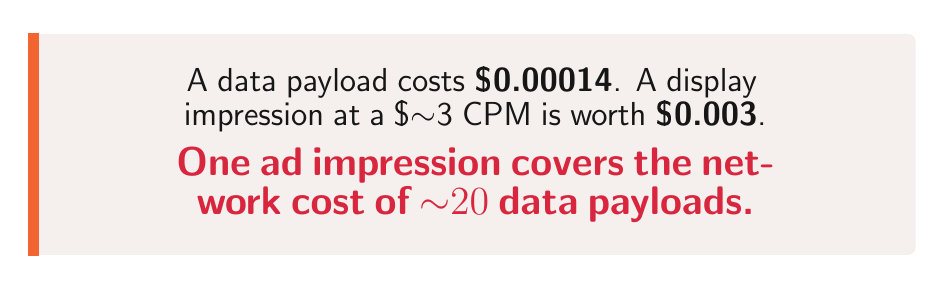
\begin{tikzpicture}
  \node[fill=f1r3mist, rounded corners=3pt, inner sep=12pt, text width=0.86\textwidth, align=center] (b) {%
    {\color{f1r3ink}\large A data payload costs \textbf{\$0.00014}. A display impression at a \$$\sim$3 CPM is worth \textbf{\$0.003}.}\\[5pt]
    {\color{f1r3red}\Large\bfseries One ad impression covers the network cost of ${\sim}20$ data payloads.}};
  \draw[line width=4pt, f1r3orange] ([xshift=2pt]b.south west) -- ([xshift=2pt]b.north west);
\end{tikzpicture}
\end{center}

Every major property is funded if a user sees just two or three ads a day --- far below real exposure --- so the typical user crosses into \emph{net-earning} portable tokens. Because impressions are themselves on-chain, fee-bearing transactions, the ad layer is self-funding volume rather than overhead, and the network still takes a thin margin at vast scale (a \$0.00002 take per payload across Gmail-scale volume is ${\sim}\$72$M/month).

This is the inversion. In incumbent Web 2.0 the user is the product: attention is extracted and the surplus is captured by the platform. Here the user covers their own cost with attention and \textbf{keeps the surplus}. Tokens earned on ad-tolerant, high-value surfaces (e.g.\ maps) pay for impression-free use of ad-averse ones (e.g.\ documents) --- a cross-subsidy carried in the \emph{user's} wallet, not wielded as the platform's lever. It is ``the community is the moat'' written as an income statement, and the structural answer to enshittification.

We enter not at full scale but through a \textbf{privacy wedge}: the ${\sim}1\%$ of users who actively want to own their data and earn from their attention. That slice is trivially funded and self-selects exactly the early adopters the pitch is built for.

% =================== ROLLOUT ===================
\section{Recommended sequence}

\begin{enumerate}[leftmargin=1.6em, itemsep=3pt]
  \item \textbf{AI (ASI Alliance) --- anchor.} Real volume hardens the dispatch/\textsc{comm} hot path; unbounded, self-funding growth.
  \item \textbf{Fintech (Boring Financial) --- margin.} Highest revenue density; builds high-assurance discipline on recoverable failures.
  \item \textbf{Medical (VA) --- annuity.} Highest per-unit margin, deployed last so the assurance and funded-floor guarantees are battle-tested first.
  \item \textbf{Music --- continuous fill.} Cold-tail packing that monetises spare capacity across the network.
  \item \textbf{Web 2.0 --- mass-market substrate.} Entered through the privacy wedge once the participatory ad rails are proven.
\end{enumerate}

The original safe-to-critical risk progression is preserved; the economic ordering simply layers on top of it, putting the unbounded, self-funding sector first and the highest-assurance sector last.

\vspace{8pt}
{\color{f1r3red}\rule{\textwidth}{1.5pt}}\\[2pt]
{\color{f1r3ash}\footnotesize All figures are engineering estimates on stated assumptions; transaction fees are levers to be replaced with real schedules from production partners. Full derivations, per-sector growth tables, and sources are in the companion working notes \emph{Rent and Shard Splitting} and \emph{Sector Economics and Go-to-Market Viability}. \quad$\cdot$\quad \textbf{F1R3FLY Industries}}

\end{document}
